\chapter{Experimental Model}
\label{ch:model}

\section{Introduction}
\label{sec:model-intro}

This chapter describes the experimental model of the study. It presents the design of the Q\&A based interactive storytelling system and of the language model at its centre, a Llama 3.2 model fine-tuned for the system's own prompts. The chapter first explains the research design: the overall architecture, the question framework, the way answers are turned into a story context and a prompt, the five-phase story model, the construction of the training data, the fine-tuning and deployment of the model, the multimodal pipelines and the implementation. It then defines the measures and statistical techniques used to analyse the results, and closes with the ethical considerations and the limitations of the design.

\section{Research Design}
\label{sec:model-design}

\subsection{Block Diagram of the Proposed System}
\label{sec:model-overall}

\Cref{fig:block} is the block diagram of the proposed system. It has three parts. The input comes from the user: the answers to the story questions, any custom answers or user-added questions, and, after each chapter, the chosen direction for the next one. The proposed system runs on the user's machine. The Q\&A module collects the answers, the context-extraction module turns them into a structured story context, and the prompt builder combines this context with the template of the current story phase, supplied by the story-flow manager, and with the previous chapters kept in memory. The fine-tuned Llama 3.2 3B model writes the chapter, and the output formatter cleans the text and adds four suggested directions. The output is the chapter with its scene illustration, narration and background music, together with the story map and character graph. The user reads the chapter and chooses the next direction, which starts the next turn.

\begin{figure}[H]
    \centering
    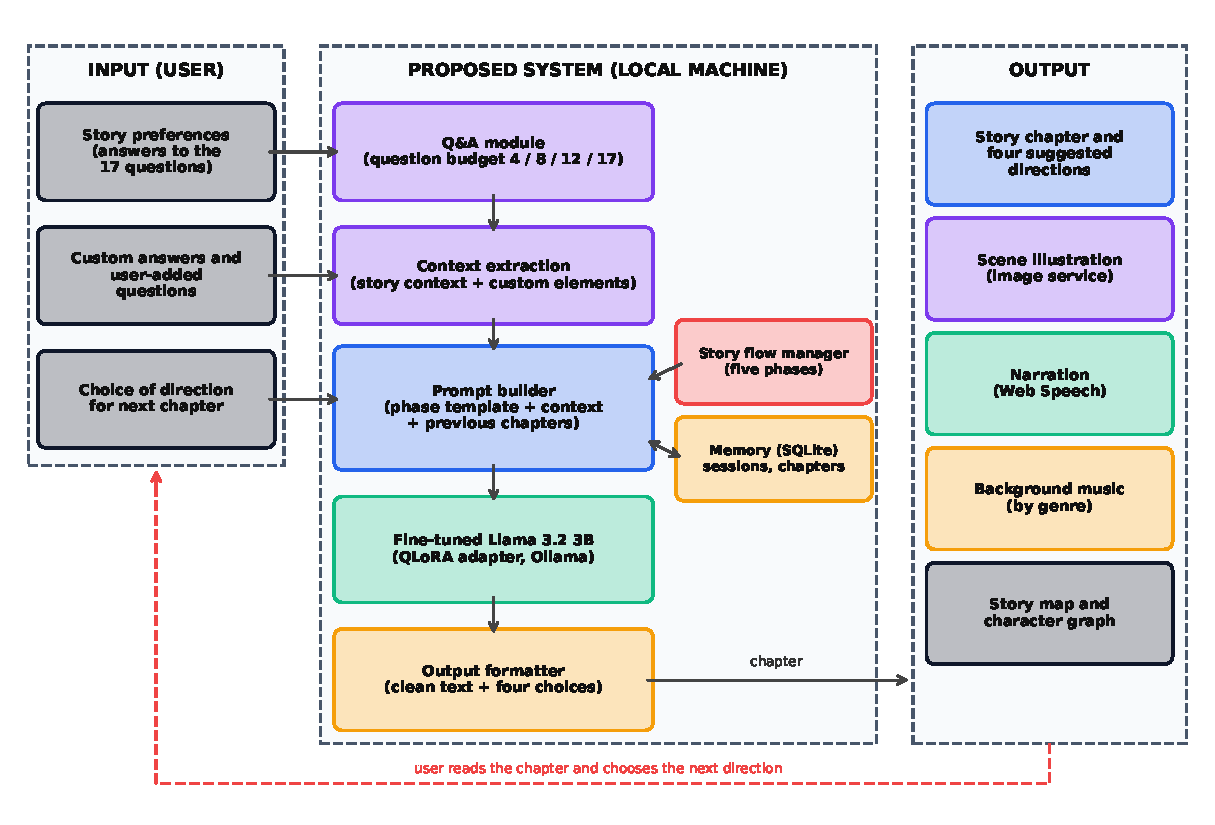
\includegraphics[width=\textwidth]{images/n07_block_diagram.pdf}
    \caption{Block diagram of the proposed system.}
    \label{fig:block}
\end{figure}

\subsection{Overall Design}

The study follows a design-and-evaluate approach. A complete system was designed and built, a language model was adapted to it, and both were evaluated: the model by a controlled comparison with its pretrained starting point on held-out data, and the framework by a user study. \Cref{fig:workflow} shows the workflow.

\begin{figure}[H]
\centering
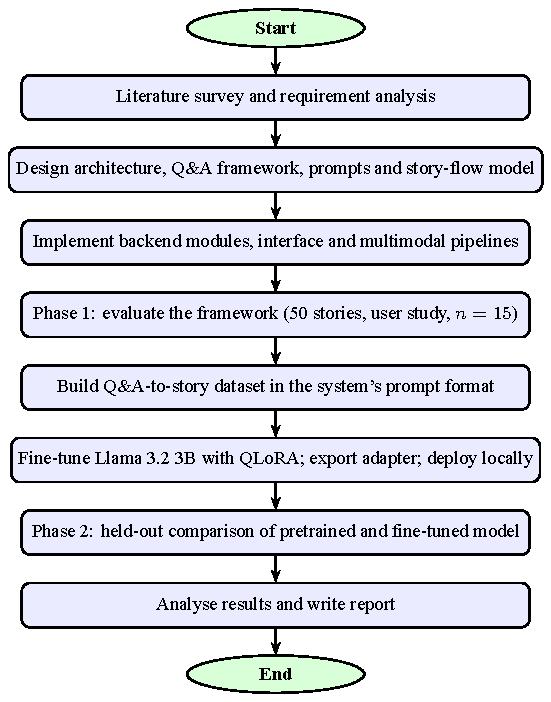
\includegraphics[width=0.6\textwidth]{images/n00_workflow.pdf}
\caption{Research workflow followed in this dissertation.}
\label{fig:workflow}
\end{figure}

The system is organised in layers, shown in \Cref{fig:arch}. The \emph{presentation layer} is a single-page web application that shows the questions, the story, the images and the analytics, and plays narration and music. The \emph{application layer} is a FastAPI server that exposes the REST endpoints and manages sessions. The \emph{modular core} contains the seven backend modules that turn answers into a story. At the bottom is the \emph{model layer}: the Ollama runtime on the same machine, which holds the pretrained Llama 3.2 3B weights and the fine-tuned adapter. Each layer depends only on the layer below it, so a module can be improved or the model replaced without touching the rest.

\begin{figure}[H]
    \centering
    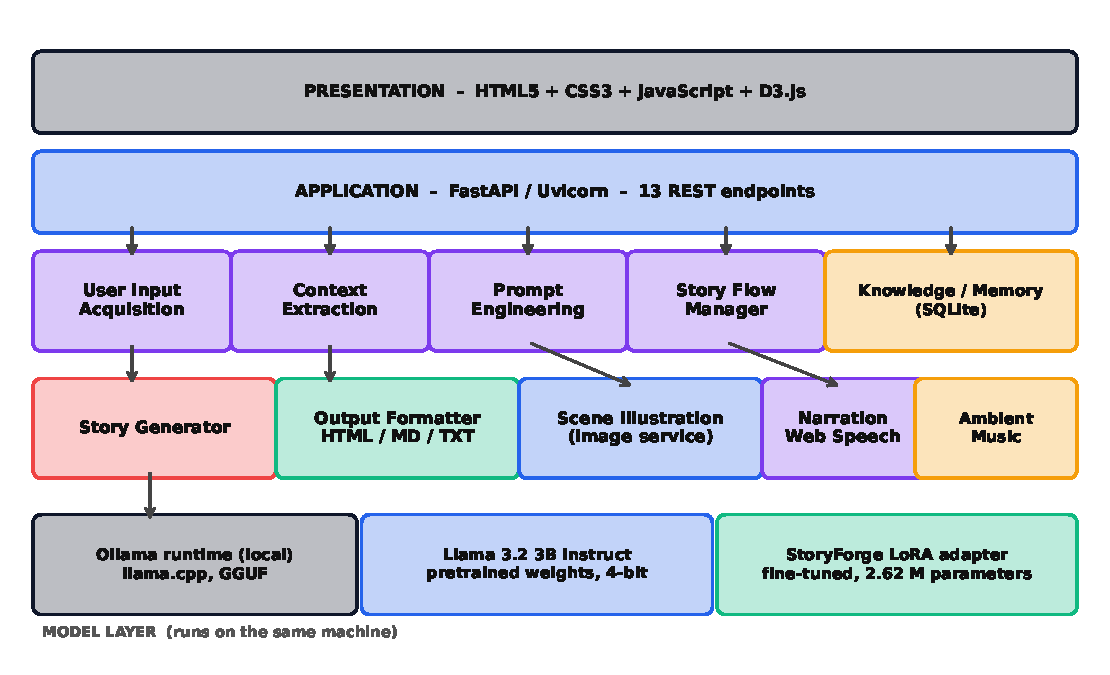
\includegraphics[width=\textwidth]{images/n01_architecture.pdf}
    \caption{Layered architecture of the proposed system.}
    \label{fig:arch}
\end{figure}

\subsection{Question-and-Answer Framework}
\label{sec:model-qa}

The elicitation protocol has seventeen questions divided among four narrative dimensions, as shown in \Cref{fig:qa}: four on the \emph{setting} (kind of world, time period, atmosphere, locations), five on the \emph{character} (the protagonist's name, personality and motivation, the allies, and the antagonist), four on the \emph{theme} (genre, emotional journey, themes and tone) and four on the \emph{plot} (type of conflict, plot style, complexity and ending).

\begin{figure}[H]
    \centering
    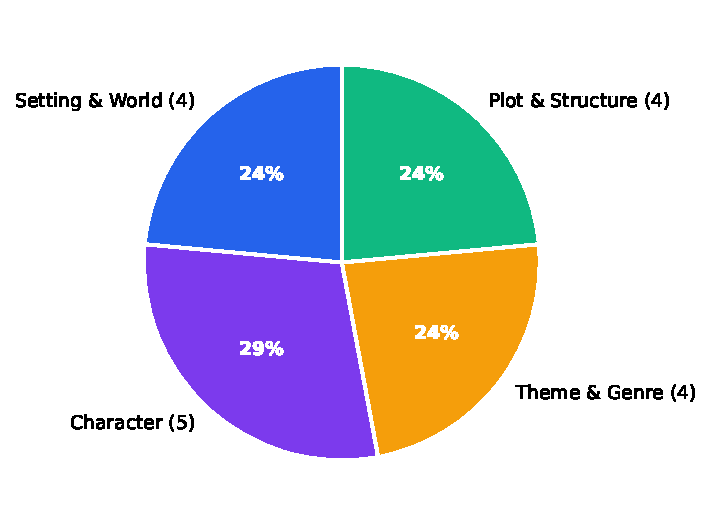
\includegraphics[width=0.62\textwidth]{images/f08_qa.pdf}
    \caption{Distribution of the 17 questions across the four dimensions.}
    \label{fig:qa}
\end{figure}

The user selects a budget of 4 (Quick), 8 (Balanced), 12 (Detailed) or 17 (Full) questions. The questions are presented in a fixed order, setting first, then character, theme and plot, and a budget of $N$ uses the first $N$ of them. A budget of 4 therefore covers the setting, 8 adds the protagonist and the allies, 12 adds the antagonist and three theme questions, and 17 covers all four dimensions. Attributes that are not asked take neutral default values in the prompt. Every question offers multiple-choice options and a ``Write my own'' option for a free-text answer. In addition, the user may add entirely new questions with their own answers.

Let $\mathcal{Q}=\{q_1,\ldots,q_{17}\}$ be the ordered question pool. The user selects a budget $N\in\{4,8,12,17\}$ and gives an answer $a_i$ to each question $q_i$ with $i \le N$. The user may also add $M$ new question-answer pairs $(\tilde q_j, \tilde a_j)$, which receive the identifiers $\mathrm{custom\_q\_}j$. The complete response set is
\begin{equation}
R = \{(q_i, a_i)\}_{i=1}^{N} \;\cup\; \{(\mathrm{custom\_q\_}j,\ \tilde a_j)\}_{j=1}^{M},
\label{eq:responses}
\end{equation}
and it is sent to the context-extraction module as a JSON dictionary.

\subsection{Context Projection and Prompt Construction}
\label{sec:model-prompt}

For each pair $(q_i,a_i)$ the context-extraction module applies a fixed projection $\pi_i$ that writes the answer into a typed field of a \texttt{StoryContext} object, for example \texttt{setting\_type}, \texttt{antagonist} or \texttt{plot\_style}. The projection uses keyword dictionaries, so that a free-text answer such as ``a haunted lighthouse'' is still mapped to a setting type. Answers whose identifiers are not known to the system, including all user-added questions, are stored word for word in a dictionary $D$ called \texttt{custom\_elements}. The final prompt $P$ is built as
\begin{equation}
P = T_{\phi}(\mathbf{c}) \oplus \sigma(D),
\label{eq:prompt}
\end{equation}
where $T_{\phi}$ is the prompt template for the current story phase $\phi$, $\mathbf{c}$ is the structured context, $\sigma$ turns the dictionary $D$ into a list of natural-language bullet points, and $\oplus$ joins the two strings. A new question added by the user thus reaches the model without any change to code or to the database schema. \Cref{fig:customq} shows this routing.

\begin{figure}[H]
    \centering
    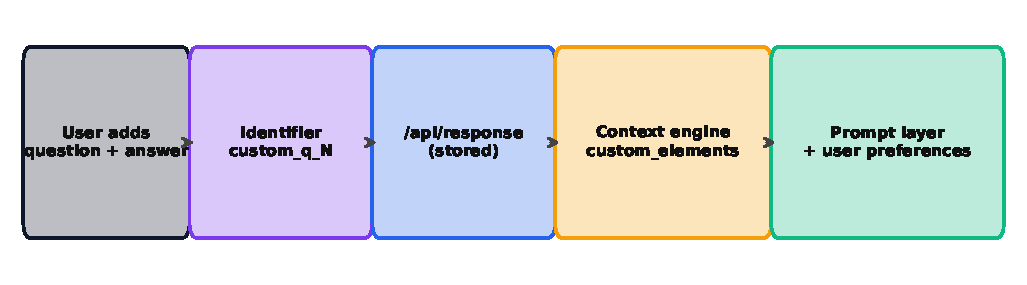
\includegraphics[width=0.95\textwidth]{images/f16_customq.pdf}
    \caption{Routing of user-added questions from the interface to the model prompt.}
    \label{fig:customq}
\end{figure}

The prompt layer has four story templates. The \emph{init} template asks for the opening of the story (about 300 to 400 words) from the full specification. The \emph{continuation} template asks for the next segment (about 250 to 350 words) from the recent story text and the direction chosen by the user. The \emph{climax} and \emph{resolution} templates ask for the turning point and the ending. A fifth template asks the model for four short choices that are offered to the user after each segment. Every request also carries a system prompt with general writing guidelines and guidance specific to the genre and the tone.

\subsection{Five-Phase Story Progression}
\label{sec:model-phases}

The story-flow manager is a finite-state machine based on Freytag's pyramid. The story moves through five phases according to its total word count, as listed in \Cref{tab:phases}. The phase and the word count together select the prompt template: the continuation template is used by default, the climax template once the story has passed 1,000 words in the rising action, and the resolution template once it has passed 1,500 words in the climax or falling action.

\begin{table}[H]
\centering
\caption{Word-count thresholds of the five story phases.}
\label{tab:phases}
\renewcommand{\arraystretch}{1.2}
\begin{tabular}{@{}lcl@{}}
\toprule
\textbf{Phase} & \textbf{Word range} & \textbf{Purpose} \\
\midrule
Introduction   & 0--400       & Establish setting and characters \\
Rising action  & 400--1200    & Develop conflict and complications \\
Climax         & 1200--1800   & Main confrontation or turning point \\
Falling action & 1800--2400   & Consequences of the climax \\
Resolution     & above 2400   & Resolve open threads and conclude \\
\bottomrule
\end{tabular}
\end{table}

The thresholds were chosen from the target length of a story and from the proportions of Freytag's model; they were not tuned on data. A story is planned for about six chapters of 300 to 400 words, that is, about 2,400 words in total. The introduction is the first chapter (up to 400 words). The rising action, which carries most of the development, is given the next two chapters (400 to 1,200 words, one third of the story), and the climax and the falling action are given about one and a half chapters each (600 words, a quarter of the story). Everything after 2,400 words belongs to the resolution. The climax prompt is requested slightly before the climax phase begins, after 1,000 words, so that the chapter that crosses the 1,200-word mark is written as the turning point.

\subsection{Dataset Construction}
\label{sec:model-dataset}

A general-purpose model has never seen the prompts of this system. To teach it, a dataset was built in which every sample is a prompt exactly as the running system produces it, paired with the story text that should follow. The construction is shown in \Cref{fig:datapipe} and has four steps.

\begin{figure}[H]
    \centering
    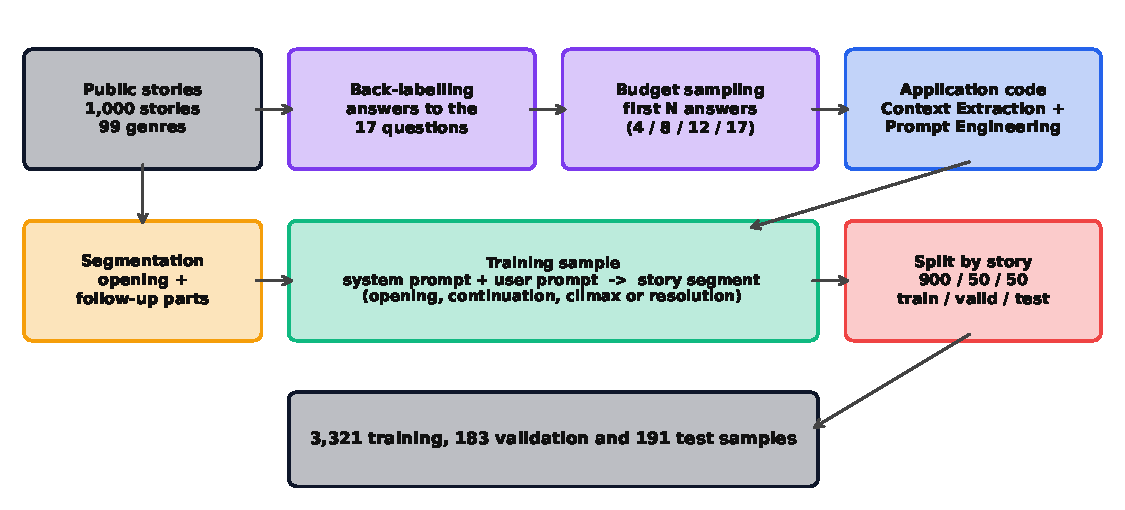
\includegraphics[width=\textwidth]{images/n02_dataset_pipeline.pdf}
    \caption{Construction of the Q\&A-to-story fine-tuning dataset.}
    \label{fig:datapipe}
\end{figure}

The source is the public collection \emph{Thousand Stories, Hundred Genres}~\cite{khan2023stories}, released under the CC-BY-2.0 licence. It contains 1,000 short stories in English, each with a title and one of 99 genre labels, with a median length of about 980 words. Chapter headings were removed from the text, because the interface adds its own chapter titles.

Each story was given answers to the system's own questions by keyword rules. The genre label decides the genre answer and, where it is explicit, the setting and the time period. Counts of keyword groups in the story text decide the locations, the protagonist's personality and motivation, the allies, the antagonist, the themes and the ending, and the conflict type follows from the antagonist. The protagonist's name is the most frequent capitalised word that is not used as a place or a group; 53 of the 1,000 stories have no clear protagonist and keep the system's default wording.

For each story a question budget was sampled with probabilities 0.50, 0.25, 0.15 and 0.10 for 17, 12, 8 and 4 questions. The first $N$ answers were passed through the system's own \texttt{ContextExtractionEngine} and \texttt{PromptEngineeringLayer}, the same code that serves the application. The system and user prompts in the dataset are therefore identical to those sent at run time, including the default values used for questions outside the budget. In half of the samples the fine-grained genre label was also supplied as a user-added question, so that the \texttt{custom\_elements} channel is represented in the data.

Each story was cut at paragraph boundaries into an opening of about 280 to 430 words and follow-up segments of about 230 to 360 words. The opening is the target of the init prompt. The last segment is the target of the resolution prompt, the one before it of the climax prompt when the story has at least four segments, and the others of the continuation prompt. As in the application, the continuation and resolution prompts carry the end of the two preceding segments, here limited to 350 words. The direction given in a continuation prompt is the one of the system's five continuation options that best describes the target segment.

The stories were divided at random into 900 for training, 50 for validation and 50 for testing. The division is by story, so that no segment of a validation or test story appears in training. \Cref{tab:dataset} gives the composition. The longest sample has 1,285 tokens, and the median is 971.

\begin{table}[H]
\centering
\caption{Composition of the fine-tuning dataset.}
\label{tab:dataset}
\renewcommand{\arraystretch}{1.2}
\begin{tabular}{@{}lrrrrrr@{}}
\toprule
\textbf{Split} & \textbf{Stories} & \textbf{Opening} & \textbf{Continuation} & \textbf{Climax} & \textbf{Resolution} & \textbf{Samples} \\
\midrule
Training   & 900 & 893 & 1,122 & 501 & 805 & 3,321 \\
Validation & 50  & 50  & 64    & 23  & 46  & 183 \\
Test       & 50  & 49  & 71    & 25  & 46  & 191 \\
\bottomrule
\end{tabular}
\end{table}

\subsection{Fine-Tuning of the Language Model}
\label{sec:model-finetune}

The base model is Llama 3.2 3B Instruct~\cite{meta2024llama32}, an open-weight decoder-only transformer with 3.21 billion parameters, 28 transformer blocks, a hidden size of 3,072 and 24 attention heads. It was chosen because it is the largest recent instruction-tuned Llama model that can be both trained and run on a laptop with 8\,GB of memory.

The model was fine-tuned with QLoRA~\cite{dettmers2023qlora} using the MLX framework~\cite{hannun2023mlx}. The base weights were kept frozen in 4-bit form. Low-rank matrices as in \Cref{eq:lora} were attached to the query, key, value and output projections of the attention layers in the top 8 of the 28 blocks, with rank $r=16$ and $\alpha=32$. This gives 2.62 million trainable parameters, 0.082\% of the model. The loss of \Cref{eq:ce} was computed on the story text only: the tokens of the system and user prompts were masked, so that the model learns to write the story and not to reproduce the prompt. \Cref{tab:hyper} lists the settings. Validation loss was measured every 150 steps on 25 validation samples, and the adapter was saved at each of these points.

\begin{table}[H]
\centering
\caption{Fine-tuning configuration.}
\label{tab:hyper}
\renewcommand{\arraystretch}{1.2}
\begin{tabular}{@{}ll@{}}
\toprule
\textbf{Setting} & \textbf{Value} \\
\midrule
Base model                  & Llama 3.2 3B Instruct, 4-bit quantised \\
Method                      & QLoRA (LoRA on frozen quantised weights) \\
Adapted matrices            & Query, key, value, output projections \\
Adapted blocks              & Top 8 of 28 \\
Rank $r$ / $\alpha$ / dropout & 16 / 32 / 0.05 \\
Trainable parameters        & 2.62 million (0.082\%) \\
Optimiser, learning rate    & Adam, $1\times10^{-4}$ \\
Batch size                  & 1, gradients accumulated over 2 steps \\
Training steps              & 600 \\
Maximum sequence length     & 1,344 tokens \\
Loss                        & Cross-entropy on story tokens only \\
Hardware                    & Apple M2, 8\,GB unified memory \\
Training time               & About one hour \\
\bottomrule
\end{tabular}
\end{table}

\subsection{Deployment of the Fine-Tuned Model}
\label{sec:model-deploy}

The application runs the model through Ollama~\cite{ollama2024}, which uses the GGUF format of llama.cpp~\cite{gerganov2023llamacpp}. The trained adapter was therefore converted to a GGUF adapter and layered on the pretrained GGUF model with a two-line model definition:

\begin{lstlisting}
FROM llama3.2:3b
ADAPTER ./storyforge-lora.gguf
\end{lstlisting}

The conversion involves two points that are easy to get wrong. First, the training framework stores the two LoRA matrices transposed with respect to GGUF and uses a direct scale factor, so both matrices are transposed and $\alpha$ is set to the scale times the rank. Second, GGUF Llama models keep the rows of the query and key projections in a different order from the weights used in training. The same row permutation therefore has to be applied to the matrix $B$ of every query and key adapter. This was checked on the base weights themselves before the adapter was written (\Cref{sec:model-verification}). The resulting model is registered under the name \texttt{storyforge}. The adapter file is 10\,MB, and the pretrained weights are shared with the base model, so both models can be offered in the interface (\Cref{fig:ui-settings}) at no extra storage cost.

\begin{figure}[H]
    \centering
    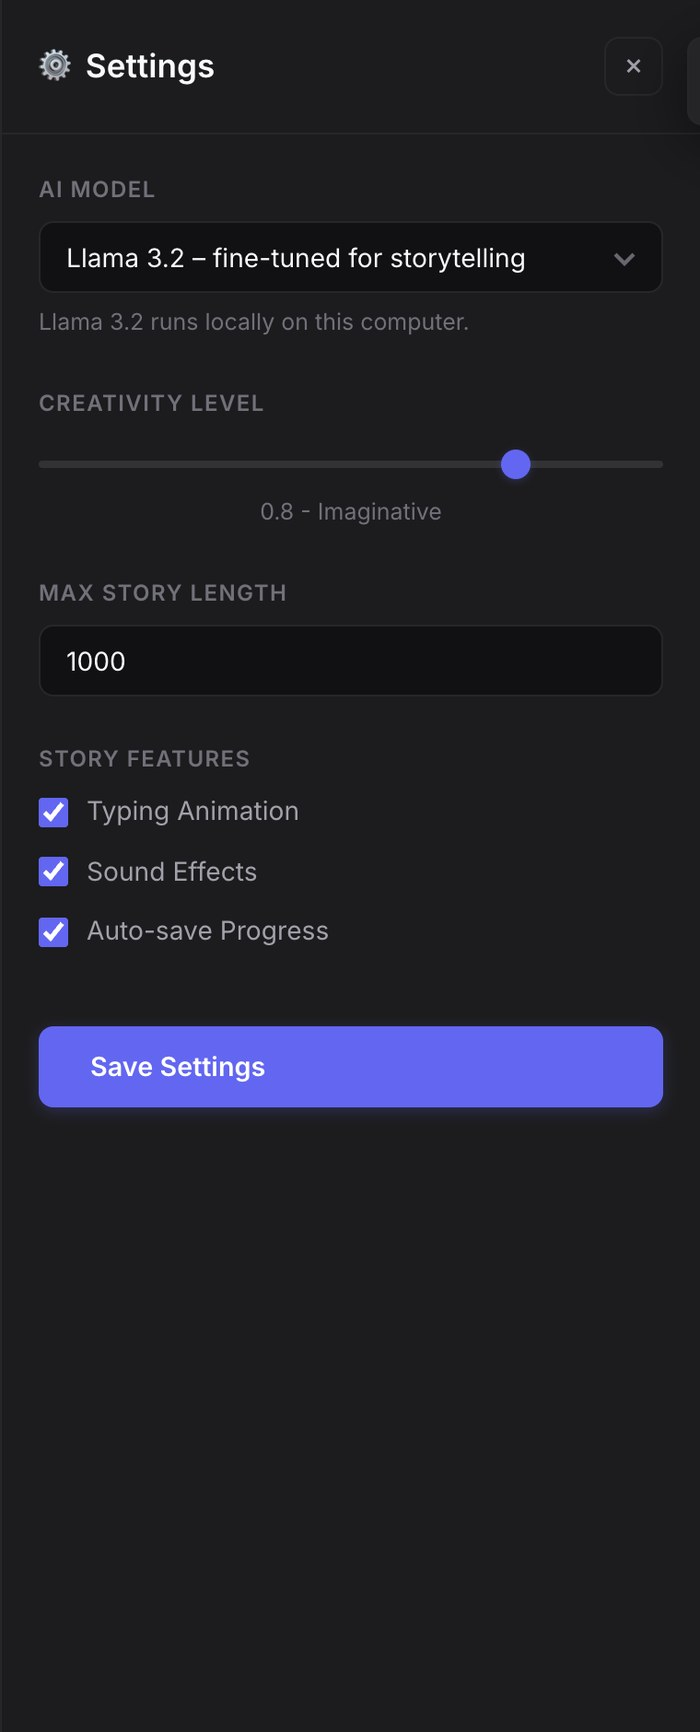
\includegraphics[width=0.5\textwidth]{images/ui_settings.jpg}
    \caption{Settings panel with the model selector: the fine-tuned model and the pretrained base.}
    \label{fig:ui-settings}
\end{figure}

\subsection{Generation Loop}
\label{sec:model-loop}

Each turn of the story follows \Cref{alg:loop}. The model receives the system prompt and one user prompt, which carries the structured context and the end of the two most recent segments. This keeps the request within the 4,096-token context configured for the local model while preserving the most recent events. Image generation starts as soon as the text is shown, so that the picture is often ready when the user finishes reading.

\begin{algorithm}[H]
\caption{Story generation loop for one turn}
\label{alg:loop}
\begin{algorithmic}[1]
\Require session $s$, structured context $\mathbf{c}$, custom elements $D$, user choice $u$ (empty on the first turn)
\Ensure formatted segment and choices for the next turn
\State $H \gets$ last two segments of session $s$
\State $\phi \gets$ current phase from total word count
\State $P \gets T_{\phi}(\mathbf{c}, H, u) \oplus \sigma(D)$
\State $y \gets \textsc{Model}(P)$ \Comment{fine-tuned Llama 3.2, local}
\State $y \gets \textsc{Format}(y)$ \Comment{clean text, style dialogue}
\State update character and plot-thread trackers with $y$
\State run continuity and pacing checks on $y$
\State save $y$ to the database; update word count and phase
\State $C \gets \textsc{Model}(\text{choice prompt for } y)$ \Comment{four options}
\State \Return $y$ and $C$; the interface then requests the scene illustration
\end{algorithmic}
\end{algorithm}

\subsection{Backend Modules}
\label{sec:model-modules}

The backend has seven modules with clear responsibilities and typed interfaces.

\textbf{User Input Acquisition} holds the question pool, serves it grouped by dimension and validates the answers. The landing page (\Cref{fig:ui-landing}) lets the user choose a budget, and the question form (\Cref{fig:ui-form}) shows each question with its options and a ``Write my own'' field.

\begin{figure}[H]
    \centering
    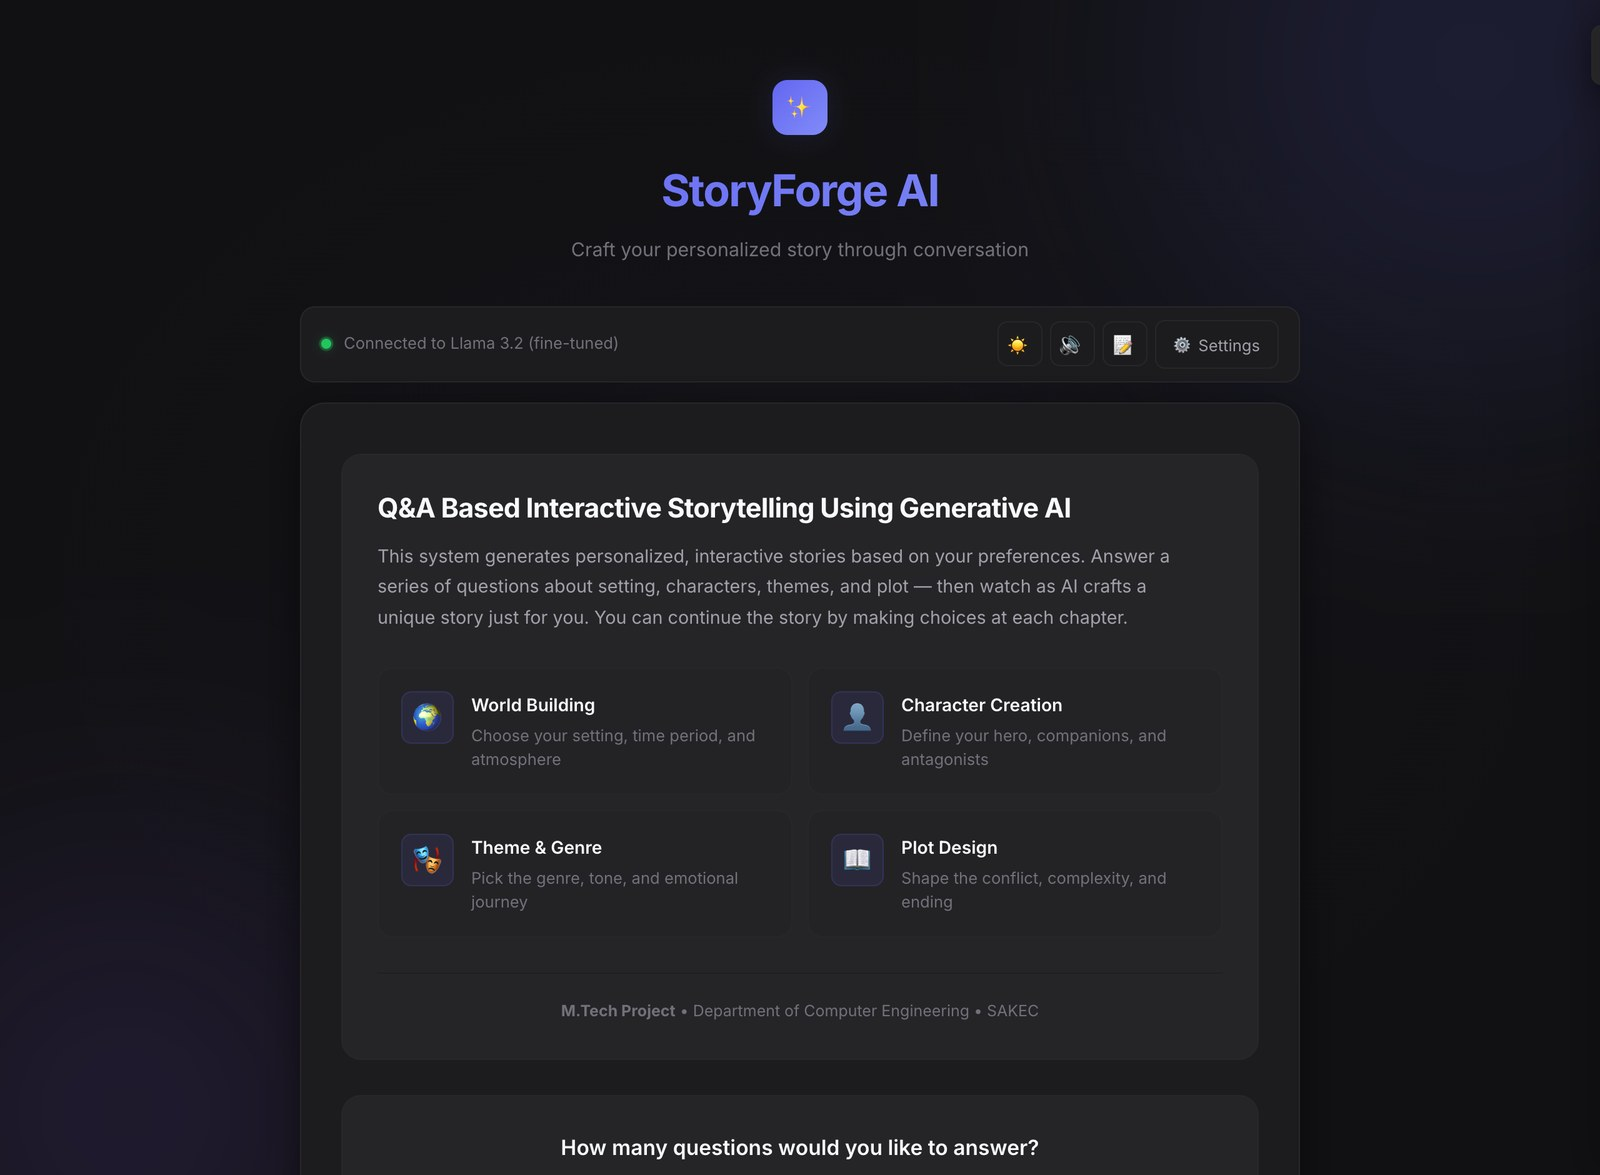
\includegraphics[width=0.8\textwidth]{images/ui_landing.jpg}
    \caption{Landing page with the choice of question budget.}
    \label{fig:ui-landing}
\end{figure}

\begin{figure}[H]
    \centering
    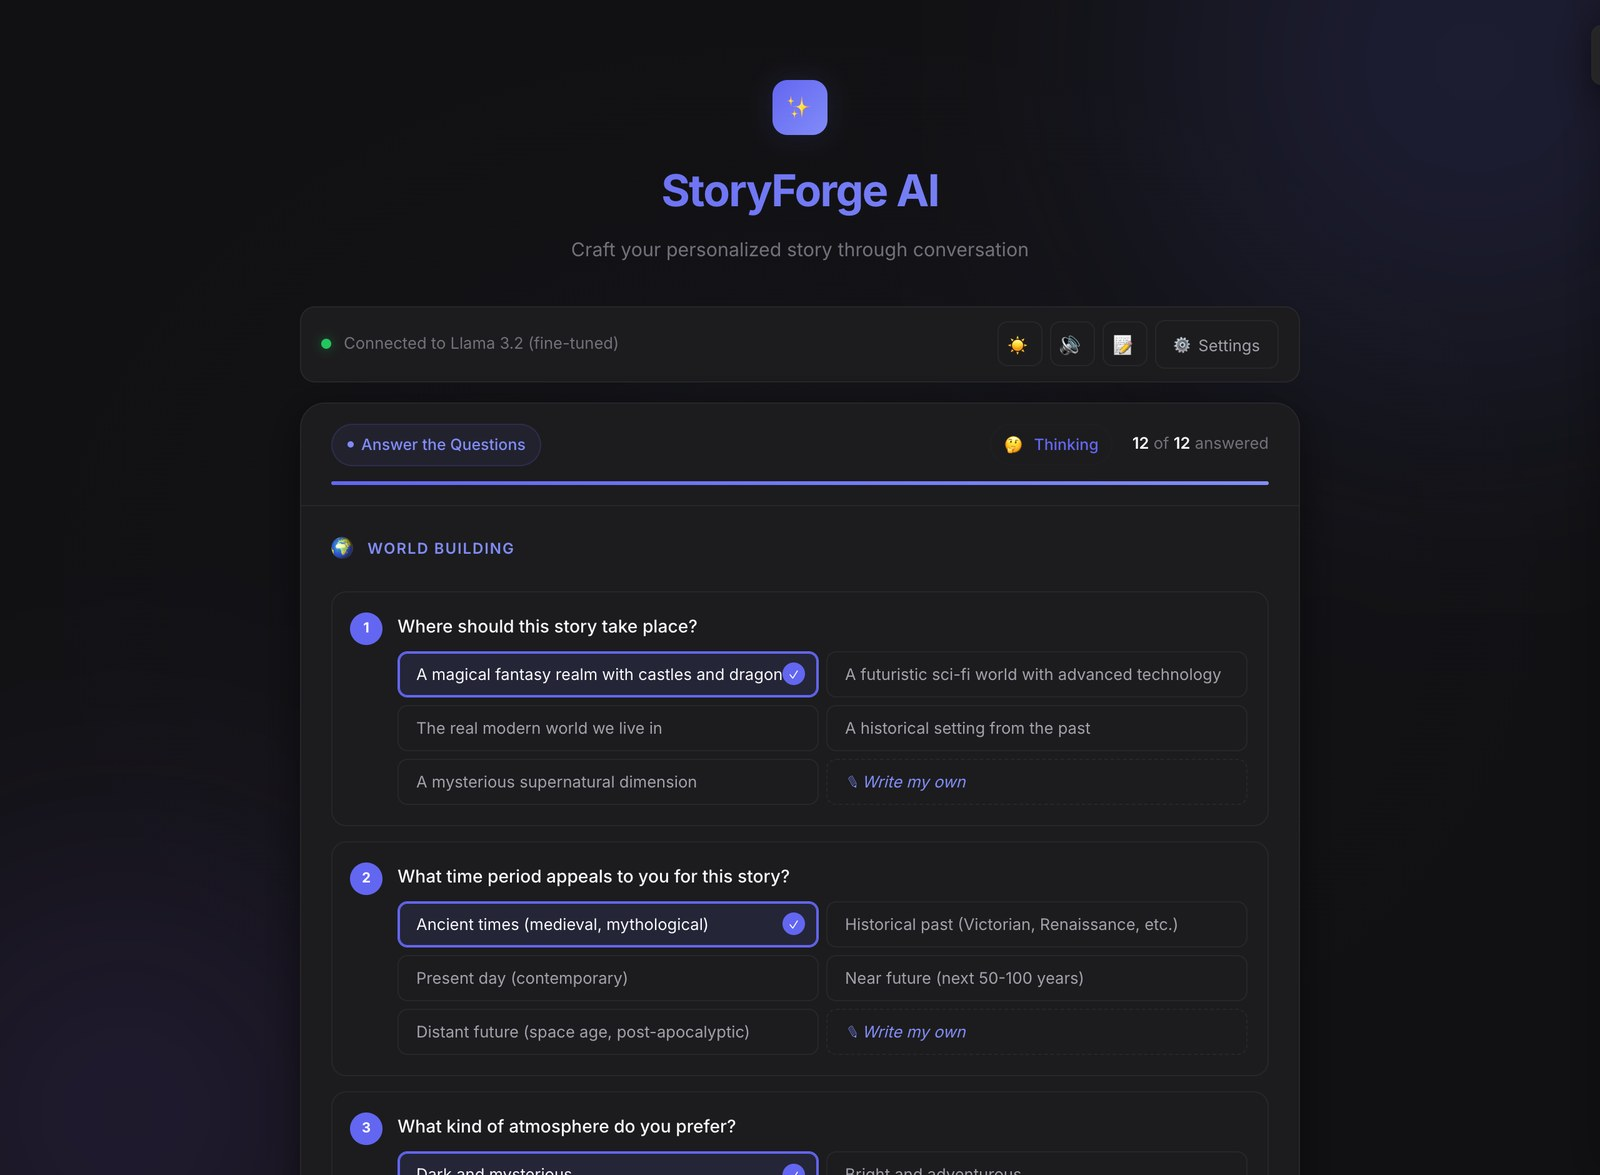
\includegraphics[width=0.8\textwidth]{images/ui_questions.jpg}
    \caption{Single-page question form with the custom-answer option.}
    \label{fig:ui-form}
\end{figure}

\textbf{Context Extraction Engine} fills the \texttt{StoryContext} object as described in \Cref{sec:model-prompt}. \textbf{Knowledge and Memory} stores sessions, answers, segments and preferences in SQLite and returns the most recent segments for the next prompt. \textbf{Prompt Engineering} holds the templates and adds genre and tone guidance. \textbf{Story Generator} sends the prompt to the model through a small client interface and returns the text; the active model can be changed at run time from the settings panel. \textbf{Story Flow Manager} implements the five-phase state machine of \Cref{sec:model-phases}. For every segment it records the word count, the characters and locations mentioned, the amount of dialogue and a keyword-based emotional tone, and it applies two rule-based checks: character continuity (a character who reappears after being marked as gone) and pacing (a long segment without dialogue). \textbf{Output Formatter} cleans the text, wraps dialogue in styled HTML and exports the full story as plain text, Markdown or HTML.

\subsection{Multimodal Pipelines}
\label{sec:model-multimodal}

For each segment, a short image prompt is built from the most visual sentence. Dialogue in quotation marks and sentences built around thought verbs are removed first, because they describe things that cannot be drawn. Each remaining sentence $s$ is scored as
\begin{equation}
\mathrm{score}(s) = 2 \cdot \mathbf{1}_{V}(s) - 2 \cdot \mathbf{1}_{T}(s) + \min\bigl(3,\ |\mathrm{ProperNouns}(s)|\bigr),
\label{eq:score}
\end{equation}
where $\mathbf{1}_V(s)$ is 1 if the sentence contains a visual verb (\emph{stood, loomed, soared, glowed, towered}, and so on) and $\mathbf{1}_T(s)$ is 1 if it contains a thought verb. The best sentence is combined with the genre, the current mood and a fixed style prefix, and the prompt is limited to 200 characters. It is sent to the Pollinations.ai image service~\cite{pollinations2024api}, as shown in \Cref{fig:imgpipe}. The service rejects bursts of parallel requests, so all image requests pass through a serial queue that sends one request at a time, waits 1.2\,s between requests and abandons a request after 35\,s. This is the only part of the system that needs a network connection and an outside service; when the service is unavailable or refuses a request, the story is shown without illustrations.

\begin{figure}[H]
    \centering
    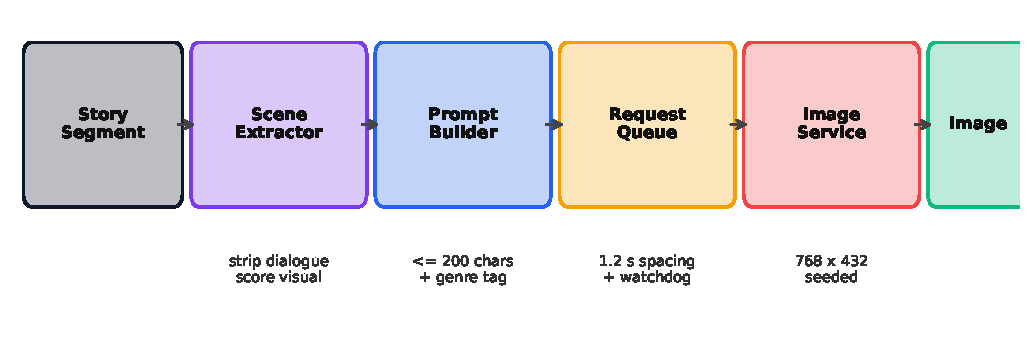
\includegraphics[width=0.95\textwidth]{images/f09_imgpipe.pdf}
    \caption{Per-segment image synthesis pipeline.}
    \label{fig:imgpipe}
\end{figure}

Narration uses the browser's built-in speech synthesis~\cite{w3c2024webspeech}. One utterance is queued per segment, with pause, resume and stop controls. Ambient music maps each genre to a royalty-free SoundHelix track~\cite{brichta2024soundhelix}, played in a loop with a 2.4\,s fade-in and a 0.8\,s fade-out (\Cref{fig:audio}).

\begin{figure}[H]
    \centering
    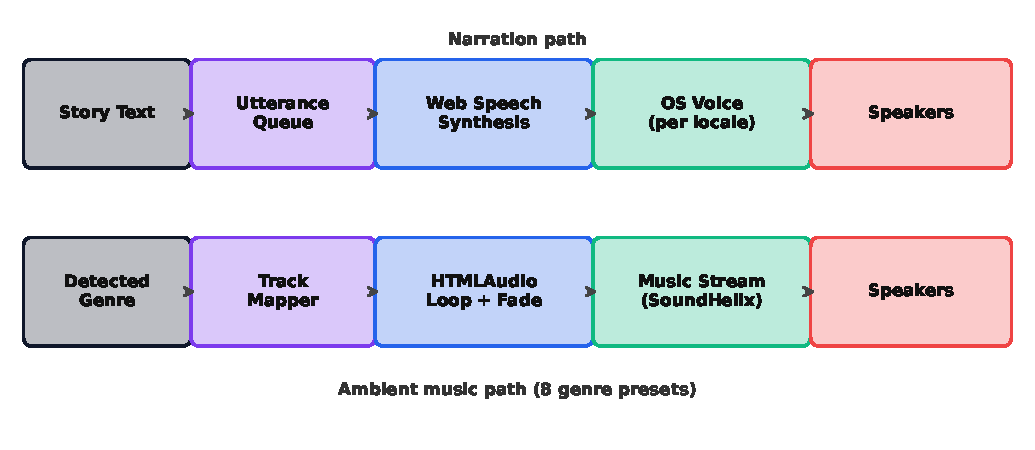
\includegraphics[width=0.95\textwidth]{images/f10_audio.pdf}
    \caption{Narration and ambient-music signal flows.}
    \label{fig:audio}
\end{figure}

The Story Map arranges the chapters as a vertical tree with the D3.js library; each node shows a preview of its chapter and the user choice that led to it. For the Character Relationship Graph, capitalised words are taken from the segment text and filtered with a stop-word list, and only names that appear at least twice are kept. The edge weight between two names is the number of segments in which both appear. Because the edges are based only on co-appearance, the interface states that the graph shows which characters appear together and not the type of relationship between them.

\subsection{Implementation}
\label{sec:model-implementation}

\Cref{tab:stack} lists the software used. All components are free, and most are open source. The SQLite database has five tables: \texttt{sessions}, \texttt{story\_segments}, \texttt{story\_context}, \texttt{qa\_history} and \texttt{user\_preferences}. The server exposes 13 REST endpoints, listed in \Cref{tab:rest}, with request and response bodies typed by Pydantic~\cite{colvin2024pydantic}. The implementation has about 3,300 lines of Python in the backend, 1,700 lines of JavaScript, 2,600 lines of CSS and 300 lines of HTML in the interface, and 750 lines of Python for the dataset, export and evaluation scripts. The source code is available as open source~\cite{jha2026repo}.

\begin{table}[H]
\centering
\caption{Technology stack.}
\label{tab:stack}
\renewcommand{\arraystretch}{1.2}
\small
\begin{tabular}{@{}lll@{}}
\toprule
\textbf{Layer} & \textbf{Technology} & \textbf{Purpose} \\
\midrule
Language model   & Llama 3.2 3B Instruct with LoRA adapter & Story generation \\
Model runtime    & Ollama (llama.cpp, GGUF)         & Local inference \\
Fine-tuning      & MLX, mlx-lm                      & QLoRA training and evaluation \\
Backend          & Python, FastAPI with Uvicorn     & REST interface and templates \\
Schemas          & Pydantic v2                      & Request and response types \\
Database         & SQLite3                          & Sessions, answers, segments \\
Frontend         & HTML5, CSS3, JavaScript          & Single-page interface \\
Visualisation    & D3.js v7                         & Story Map, Character Graph \\
Image service    & Pollinations.ai                  & Scene illustrations \\
Speech           & W3C Web Speech Synthesis         & Narration \\
Ambient audio    & HTMLAudio with SoundHelix        & Genre music \\
\bottomrule
\end{tabular}
\end{table}

\begin{table}[H]
\centering
\caption{REST endpoints of the application server.}
\label{tab:rest}
\renewcommand{\arraystretch}{1.15}
\small
\begin{tabular}{@{}lcl@{}}
\toprule
\textbf{Endpoint} & \textbf{Method} & \textbf{Purpose} \\
\midrule
\texttt{/}                           & GET    & Web interface \\
\texttt{/api/status}                 & GET    & Check that the model is available \\
\texttt{/api/session/new}            & POST   & Create a new session \\
\texttt{/api/questions/all}          & GET    & All questions, grouped by dimension \\
\texttt{/api/question/next}          & GET    & Next question (sequential mode) \\
\texttt{/api/response}               & POST   & Submit an answer \\
\texttt{/api/story/generate}         & POST   & Generate the first segment \\
\texttt{/api/story/continue}         & POST   & Continue from a user choice \\
\texttt{/api/story/full/\{id\}}      & GET    & Full story of a session \\
\texttt{/api/story/download/\{id\}}  & GET    & Export as TXT, MD or HTML \\
\texttt{/api/settings}               & POST   & Change model or temperature \\
\texttt{/api/session/\{id\}/summary} & GET    & Session statistics \\
\texttt{/api/session/\{id\}}         & DELETE & End a session \\
\bottomrule
\end{tabular}
\end{table}

\subsection{Experimental Setup}
\label{sec:model-setup}

The evaluation was carried out in two phases, and the results are kept apart throughout this report.

Phase 1 evaluated the framework. During its development, 50 stories were generated across six genres and all four question budgets, and a user study was conducted with 15 participants (8 male, 7 female, aged 22 to 35, with technical and non-technical backgrounds). Each participant created two stories, giving 30 stories, and rated each on a five-point Likert scale for coherence, creativity, engagement and consistency, together with their satisfaction with each feature. The character extractor was evaluated against 50 hand-annotated segments, and the image queue was tested under parallel load. In this phase the fine-tuned model did not yet exist, and the language model was the pretrained Llama 3.1 8B Instruct model, used as a hosted model. The ratings of this phase therefore describe the framework with a pretrained model, and they are not claimed for the fine-tuned model.

Phase 2 evaluated the fine-tuned model, which was compared with its pretrained starting point, Llama 3.2 3B Instruct, in two ways. First, the loss of both models was computed on all 191 samples of the held-out test set. Second, both models generated story text, through the same runtime and with the application's own settings (temperature 0.8, top-$p$ 0.9, at most 1,000 new tokens, a 4,096-token context), for 69 held-out prompts: all 49 opening prompts of the test set and the first 20 continuation prompts. The same random seed was used for both models on each prompt. All phase-2 training and measurements were made on an Apple M2 laptop with 8\,GB of unified memory running macOS, with no other model loaded.

\section{Data Analysis Techniques}
\label{sec:model-analysis}

\subsection{Evaluation Metrics}

The following measures are used.

\begin{itemize}
    \item \textbf{Loss and perplexity.} The cross-entropy of \Cref{eq:ce} on the story tokens of a held-out sample, and its exponential. Totals are weighted by the number of story tokens. Lower values mean that the model assigns higher probability to the reference story.
    \item \textbf{Prompt-adherence measures} on generated text: the number of words; the share of outputs within $\pm 25\%$ of the requested length range; the share that begin directly with story text, with no title, heading or comment about the task; the share that mention the protagonist named in the prompt; and the share that end in a complete sentence. The ratio of distinct word pairs to all word pairs (distinct-2) is reported as a measure of lexical variety.
    \item \textbf{Generation speed and latency.} New tokens per second as reported by the runtime, and the time in seconds to produce a segment.
    \item \textbf{Likert score.} The mean rating from 1 (poor) to 5 (excellent) for each dimension of the user study.
    \item \textbf{Precision, recall and $F_1$} for character extraction, with
    \begin{equation}
    P = \frac{TP}{TP+FP}, \qquad R = \frac{TP}{TP+FN}, \qquad F_1 = \frac{2PR}{P+R}.
    \end{equation}
\end{itemize}

\subsection{Analysis Procedure}

The two models are compared on the same samples, so paired tests are used. For the held-out loss, the difference between the pretrained and the fine-tuned model is computed for each sample. The mean difference is reported with a 95\% confidence interval obtained by bootstrap resampling (10,000 resamples), together with a paired $t$-test, the Wilcoxon signed-rank test, which makes no assumption of normality, and Cohen's $d$ as a measure of effect size. Several samples come from the same story and are not independent, so the analysis is repeated at the level of stories, after averaging the samples of each story. For the generated text, proportions are compared with McNemar's exact test on the paired outcomes and word counts with the Wilcoxon signed-rank test. A significance level of 0.05 is used.

\subsection{Verification of the Measurement Pipeline}
\label{sec:model-verification}

Two checks were made before the results were collected. The first concerns the conversion of the adapter described in \Cref{sec:model-deploy}. The query, key, value and output projection weights of two blocks were read from the GGUF base model and from the training copy of the same model and compared. For the value and output projections the correlation between the two copies was 0.99 as stored. For the query and key projections it was 0.01 as stored and 0.99 after the row permutation, which confirms both that the two files hold the same model and that the permutation applied to the adapter is the correct one. The runtime also reported loading all 64 adapter matrices. The second check concerns the application path. A complete session, from creating a session and submitting 17 answers and a user-added question to generating an opening and a continuation, was run through the REST interface with the fine-tuned model, and the interface was exercised in a browser, including the switch between the two models.

\section{Ethical Considerations}
\label{sec:model-ethics}

Generated stories may contain unsuitable content if the user asks for it or if the model produces it by mistake. The base model was released with its own safety training, but the system applies no additional content filter, and it is not intended for unsupervised use by children.

The fine-tuning data is a public dataset released under a licence that permits reuse with attribution, and it is cited where it is used. The dataset card does not document how the stories were written, so the data may itself contain machine-written text; this is stated as a limitation and not concealed. The base model is used under its community licence. Because the language model runs on the user's own machine, the answers a user gives are not sent to any third party. The image prompt for each segment, a short description of a scene, is sent to the online image service.

Participants in the user study took part voluntarily, gave informed consent and could stop at any time. No personal data beyond the story answers was collected, and results are reported only as averages. The held-out test stories were not used in training or in choosing the training settings, and the results of the two evaluation phases are reported separately so that ratings obtained with one model are not attributed to another.

\section{Limitations}
\label{sec:model-limitations}

The training data comes from one collection of 1,000 stories, and the answers attached to each story were produced by keyword rules, so some of them are wrong. The model was trained once, for 600 steps, without a search over training settings. The phase-1 user study used a pretrained model, so the fine-tuned model has not been rated by users.
